\documentclass[a4paper, 11pt]{book}
\usepackage[utf8]{inputenc}
\usepackage[T1]{fontenc}
\usepackage{graphicx}
\usepackage{xcolor}
\usepackage{geometry}
\usepackage{lmodern}
\usepackage{pagecolor}
\usepackage{tikz}
\usepackage{fancyhdr}
\usepackage{tikz-3dplot}
\usepackage{amsmath}    
\usepackage{multicol}  
\usepackage{physics}    
\usetikzlibrary{arrows.meta, angles, quotes}
\pagecolor{gray!10}

\geometry{
  left=3cm,
  right=3cm,
  top=2.5cm,
  bottom=2.5cm,
  bindingoffset=0cm
}

\definecolor{blue}{RGB}{20,62,114}
\definecolor{red}{RGB}{180,35,40}
\definecolor{gray}{RGB}{80,80,80}

\begin{document}

\begin{titlepage}
    \thispagestyle{empty}
    
    \begin{center}
        \vspace*{1.5cm}

        \hrulefill \\ [.8em]

        {\fontsize{36}{44}\bfseries Calculus-Based}
        
        \vspace{0.45cm}
        
        \begin{minipage}{0.9\textwidth}
            \centering
            {\fontsize{42}{50}\selectfont\color{blue}\bfseries
            Mechanics \color{black}\&\vspace*{0.3cm}
            \color{red}Electromagnetics}
        \end{minipage} \\ [.25em]

        \hrulefill \\

        \vspace{.8cm}
    
        {\Large\color{gray}\textit{Summer of Making}}\\[0.3em]
        {\large\color{gray}HackClub}
        
    
		\vspace{3cm}
        
        \begin{minipage}{0.8\textwidth}
            \centering
            \includegraphics[height=5cm]{latex.png}\hspace{1.5cm}
            \includegraphics[height=5cm]{em1.png}
        \end{minipage}
        
        \vspace{3.7cm}
        
        {\small June 2025}
        
    \end{center}
\end{titlepage}

\clearpage
\thispagestyle{empty}
\begin{center}
	\vspace*{5cm}
	{\Huge\bfseries Preface}
	\vspace{1.0cm}

	\rule{0.5\linewidth}{0.4pt}

	\vspace{1.5cm}
	
	\begin{minipage}{0.8\textwidth}
		\Large\centering Special thanks to Mr. H and Mr. G who have 
		\\[0.2em] introduced me to the big wide world of physics.
		\\[0.2em] This book's philosophy is based off their teachings.
		\\[0.2em] While fundamental theorems will be listed in the  
		\\[0.2em] following chapters, the ultimate goal is to provide the 
		\\[0.2em] intuition for physics through mathematical reasoning. 
		\\[0.2em] Emphasis, therefore, will be placed on understanding 
		\\[0.2em] that builds upon previous concepts.
		
		
	\end{minipage}
\end{center}

\let\cleardoublepage\clearpage

\tableofcontents

% VECTORS
\chapter{Vectors and Math}

\section{What is a vector?}
A vector is a quantity with both magnitude and direction. We represent them as arrows wherein:

\begin{itemize}
\item Length indicates magnitude
\item Orientation indicates direction
\end{itemize}

% figure 1.1
\begin{figure}[h]
\centering

\begin{tikzpicture}[>=Stealth, scale=1.5]

\draw[->] (0,0,0) -- (3,0,0) node[right]{$x$};
\draw[->] (0,0,0) -- (0,3,0) node[above]{$z$};
\draw[->] (0,0,0) -- (0,0,3) node[below left]{$y$};

\draw[->, ultra thick, blue] (0,0,0) -- (2,2,1.5) 
	node[above right]{$\vec{A}$};

\draw[dashed, gray] (2,2,1.5) -- (2,0,1.5);
\draw[dashed, gray] (2,0,1.5) -- (2,0,0); 
\draw[dashed, gray] (2,0,1.5) -- (0,0,1.5); 

\end{tikzpicture}

\caption{Vector $\vec{A}$ with components $A_x$, $A_y$, and $A_z$ in 3D space}

\end{figure}


\noindent The length of a vector is traditionally denoted with double vertical bars, \textbf{|| ||}, and can be determined either
graphically or analytically. This leads us to our first equation.

\begin{equation}
\label{eq:vectorlength}
||\vec{A}|| = \sqrt{A_x^2 + A_y^2 + A_z^2}
\end{equation}

Equation~\ref{eq:vectorlength} is a representation of the Pythagorean Theorem.

\vspace{.4cm}
\noindent The direction of a vector is given by $\theta$ or $\phi$ and can be found physically such as with a protractor or analytically.

\begin{equation}
\label{eq:vectorangle}
\phi = \arctan\left(\frac{A_y}{A_x}\right)
\end{equation}

Angles in 2D space are often measured relative to the positive x-axis.

\subsection{Vector Operations}

\subsubsection{Addition}
Vector addition is commutative and follows the \textbf{parallelogram rule}:
\[
\vec{A} + \vec{B} = \vec{C}
\]
\[
\vec{C} = (A_x + B_x)\hat{i} + (A_y + B_y)\hat{j} + (A_z + B_z)\hat{k}
\]

% figure 1.2
\begin{figure}[h]
\centering
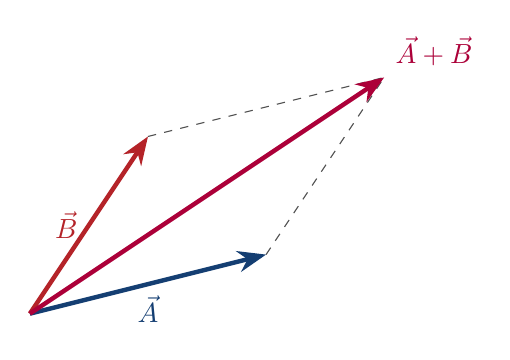
\begin{tikzpicture}[>=Stealth, scale=1.5]
    
    \draw[->, ultra thick, blue] (0,0) -- (2,0.5) node[midway, below]{$\vec{A}$};
    \draw[->, ultra thick, red] (0,0) -- (1,1.5) node[midway, left]{$\vec{B}$};
    
    \draw[dashed, gray] (2,0.5) -- (3,2);
    \draw[dashed, gray] (1,1.5) -- (3,2);
    
    \draw[->, ultra thick, purple!90!black] (0,0) -- (3,2) node[at end, above right]{$\vec{A}+\vec{B}$};
    
\end{tikzpicture}
\caption{The sum of $\vec{A}$ and {$\vec{B}$ using the parallelogram rule.}}
\end{figure}

\noindent The "tip-to-tail" method can also be used by placing the tip of one vector at the tail of the other vector
and forming the resultant triangle. Try it out for yourself! 

\subsubsection{Subtraction}
To perform vector subtraction, it is useful to consider the following example:
\[
\vec{A} - \vec{B} = \vec{A} + (-\vec{B})
\]
We treat the operation as if it were addition but flip the sign of $\vec{B}$. Graphically, this means rotating the 
vector 180$^{\circ}$.

\subsubsection{Multiplication}
There are two types of vector multiplication. 

\begin{itemize}
	\item Dot Product:
		The dot product finds the component of $\vec{A}$ in the direction of $\vec{B}$. 
		
        \begin{equation}
        \label{eq:dotproduct}
        \vec{A} \cdot \vec{B} = |A||B|\cos\theta
        \end{equation}

	\item Cross Product:
        The cross product finds the component of $\vec{A}$ orthogonal to $\vec{B}$. 
        
        \begin{equation}
        \label{eq:crossproduct}
        \vec{A} \times \vec{B} = |A||B|\sin\theta
        \end{equation}

\end{itemize}

\noindent Note that vector division is not defined.

\newpage
\section{Coordinate Systems}
It is useful and even necessary at times to establish a consistent coordinate system.
An example is the right-hand coordinate system. Extend your hand in the direction of the positive x-axis.
Now curl your fingers toward the positive y-axis. Finally, stick out your thumb. It should point toward the
positive z-axis.

% figure 1.3
\begin{figure}[h]
\centering
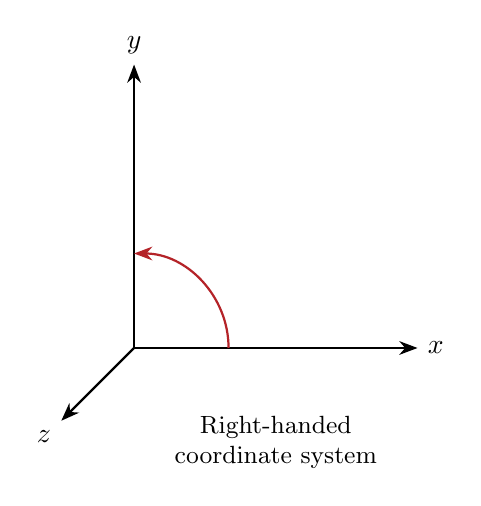
\begin{tikzpicture}[>=Stealth, scale=1.2]

\draw[->, thick] (0,0,0) -- (3,0,0) node[right]{$x$};
\draw[->, thick] (0,0,0) -- (0,3,0) node[above]{$y$};
\draw[->, thick] (0,0,0) -- (0,0,2) node[below left]{$z$};

\draw[->, thick, red] (1,0,0) arc (0:90:1);

\node[align=center, font=\small] at (1.5,-1) {Right-handed\\coordinate system};

\end{tikzpicture}
\caption{Right-Hand Coordinate System}
\end{figure}

\noindent Other coordinate systems will be discussed in separate chapters, but
this system can represent most systems in undergraduate mechanics and electromagnetics.

\section{Math}
The following section will list important mathematical foundations used in basic physics problems.

\begin{multicols}{2}
\begin{itemize}
\item \textbf{Derivative Definition}
      \[\frac{df}{dx} = \lim_{h\to 0}\frac{f(x+h)-f(x)}{h}\]

\item \textbf{Product Rule}
      \[\frac{d}{dx}(uv) = u\frac{dv}{dx} + v\frac{du}{dx}\]

\item \textbf{Chain Rule}
      \[\frac{df(g(x))}{dx} = f'(g(x))g'(x)\]

\item \textbf{Quotient Rule}
      \[\frac{d}{dx}\left(\frac{u}{v}\right) = \frac{v\frac{du}{dx} - u\frac{dv}{dx}}{v^2}\]

\item \textbf{Taylor Series}
      \[f(x) = \sum_{n=0}^\infty \frac{f^{(n)}(a)}{n!}(x-a)^n\]

\item \textbf{Power Rule}
      \[\frac{d}{dx}(x^n) = nx^{n-1}\]

\item \textbf{Derivative of $e^{ax}$}
      \[\frac{d}{dx}e^{ax} = ae^{ax}\]

\item \textbf{Derivative of $\ln(ax)$}
      \[\frac{d}{dx}\ln(ax) = \frac{1}{x}\]

\item \textbf{Derivative of sin}
      \[\frac{d}{dx}\sin(ax) = a\cos(ax)\]

\item \textbf{Derivative of cos}
      \[\frac{d}{dx}\cos(ax) = -a\sin(ax)\]

\item \textbf{Integral of $x^n$, n $\neq$ -1}
      \[\int x^n \,dx = \frac{x^{n+1}}{n+1} + C\]

\item \textbf{Integral of $e^{ax}$}
      \[\int e^{ax} \,dx = \frac{1}{a}e^{ax} + C\]

\item \textbf{Integral of $\ln(ax)$}
      \[\int \frac{1}{x+a} \,dx = \ln|x+a| + C\]

\item \textbf{Integral of sin}
      \[\int \sin(ax) \,dx = -\frac{1}{a}\cos(ax) + C\]

\item \textbf{Integral of cos}
      \[\int \cos(ax) \,dx = \frac{1}{a}\sin(ax) + C\]

\item \textbf{Circumference of Circle}
      \[C = 2\pi r\]

\item \textbf{Arc Length of Circle}
      \[s = r\theta\]

\item \textbf{Volume of Cylinder}
      \[\pi r^2 l\]

\item \textbf{Volume of Sphere}
      \[\frac{4}{3}\pi r^3\]

\item \textbf{Surface Area of Cylinder}
      \[2\pi rl\]


\item \textbf{Surface Area of Sphere}
      \[4\pi r^2\]

\item \textbf{Double Angle Identity}
      \[\sin(2\theta) = 2\sin\theta\cos\theta \]
      
\item \textbf{Sin and Cos Identity}
      \[\sin^2(\theta) + \cos^2(\theta) = 1\]

\item \textbf{Log Identity}
      \[\log(a \cdot b^x) = \log a + x \log b\]

\end{itemize}
\end{multicols}


\chapter{Kinematics}
\section{Describing Motion}
Kinematics is the study of motion. Generally, we discuss objects, otherwise known as projectiles,
moving at constant \textbf{velocity} or \textbf{acceleration}. These are vectors that can
indicate how position changes with time. In other words:

\begin{equation}
    \label{eq:velocity}
    \vec{v} = \frac{dx}{dt}
\end{equation}

\begin{equation}
    \label{eq:acceleration}
    \vec{a} = \frac{d^2x}{dt^2}
\end{equation}

\begin{figure}[h]
\centering
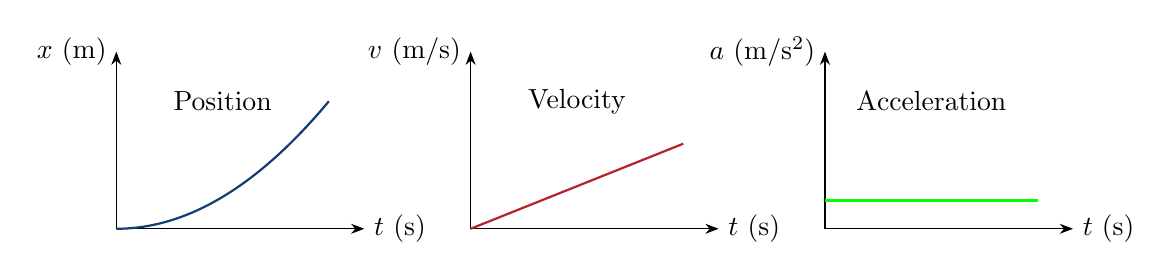
\begin{tikzpicture}[>=Stealth, scale=0.9]

\begin{scope}[shift={(0,0)}]
\draw[->] (0,0) -- (3.5,0) node[right]{$t$ (s)};
\draw[->] (0,0) -- (0,2.5) node[left]{$x$ (m)};
\draw[thick,blue,domain=0:3,smooth] plot (\x,{0.2*\x*\x});
\node at (1.5,1.8) {Position};
\end{scope}


\begin{scope}[shift={(5,0)}]
\draw[->] (0,0) -- (3.5,0) node[right]{$t$ (s)};
\draw[->] (0,0) -- (0,2.5) node[left]{$v$ (m/s)};
\draw[thick,red,domain=0:3,smooth] plot (\x,{0.4*\x});
\node at (1.5,1.8) {Velocity};
\end{scope}


\begin{scope}[shift={(10,0)}]
\draw[->] (0,0) -- (3.5,0) node[right]{$t$ (s)};
\draw[->] (0,0) -- (0,2.5) node[left]{$a$ (m/s$^2$)};
\draw[thick,green,domain=0:3,smooth] plot (\x,{0.4});
\node at (1.5,1.8) {Acceleration};
\end{scope}
\end{tikzpicture}
\caption{Side by Side Position, Velocity, and Acceleration Graphs}
\end{figure}
x(t) exhibits quadratic growth, v(t) linear, a(t) acceleration constant.



\section{Constant Acceleration Kinematics}
From the fundamental definitions:

\begin{align*}
v &= v_0 + at \\
x &= x_0 + v_0t + \frac{1}{2}at^2 \\
v^2 &= v_0^2 + 2a\Delta x
\end{align*}


\section{Graphical Analysis}



\section{Projectile Motion}
Decomposed into independent horizontal/vertical motions:

\begin{align*}
x(t) &= x_0 + v_{x0}t \\
y(t) &= y_0 + v_{y0}t - \frac{1}{2}gt^2 \\
\text{Range} &= \frac{v_0^2\sin 2\theta}{g} \quad (\text{for } y_0=0)
\end{align*}

\begin{figure}[h]
\centering
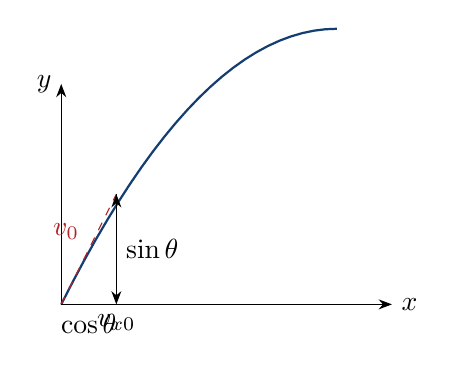
\begin{tikzpicture}[>=Stealth, scale=0.7]
\draw[->] (0,0) -- (6,0) node[right]{$x$};
\draw[->] (0,0) -- (0,4) node[left]{$y$};
\draw[thick,blue,domain=0:5] plot (\x,{2*\x - 0.2*\x*\x});
\draw[dashed,red] (0,0) -- (1,2) node[midway,above left]{$v_0$};
\draw[dashed] (1,2) -- (1,0) node[below]{$v_{x0}$};
\draw[dashed] (0,0) -- (1,0) node[midway,below]{$\cos\theta$};
\draw[<->] (1,0) -- (1,2) node[midway,right]{$\sin\theta$};
\end{tikzpicture}
\caption{Projectile motion components showing velocity decomposition}
\end{figure}

\end{document}

